\section{Тестирование метода}

\subsection{Распространение продольной волны (P-волны)}
Пусть плоская P-волна в среде распространяется вдоль оси z. В этом случае аналитическое решение соответствующего одномерного уравнения дает следующие соотношения на параметры волны:
\begin{itemize}
\item $v_z=-f(z)\sqrt{\frac{\lambda+2\mu}{\rho}}=C_p$;
\item $v_x=v_y=0$;
\item $\sigma_{zz}=f(z)(\lambda+2\mu)$;
\item $\sigma_{xx}=\sigma_{yy}=f(z)\lambda$;
\item $\sigma_{ij}=0$ для $i \neq j$.
\end{itemize}
Здесь $f(z)$ - произвольная функция, зависящая только от z и задающая форму волны.
Для расчёта распространения P-волны в кубе были использованы следующие безразмерные параметры: 
\begin{itemize}
\item размер расчётной области: 50x50x50;
\item $\lambda=70000$;
\item $\mu=10000$;
\item $\rho=1$.
\end{itemize}
На графиках (см. рис.
\ref{pic:p_wave_1}-\ref{pic:p_wave_15}) представлены результаты численного расчёта. Получено совпадение параметров волны с аналитическим решением:
\begin{itemize}
\item $v_z=C_p=300$;
\item $\frac{\sigma_{zz}}{\sigma_{xx}}=\frac{\sigma_{zz}}{\sigma_{yy}}=\frac{\lambda+2\mu}{\lambda}=\frac{9}{7}$.
\end{itemize}

\begin{figure}[htp]
\centering
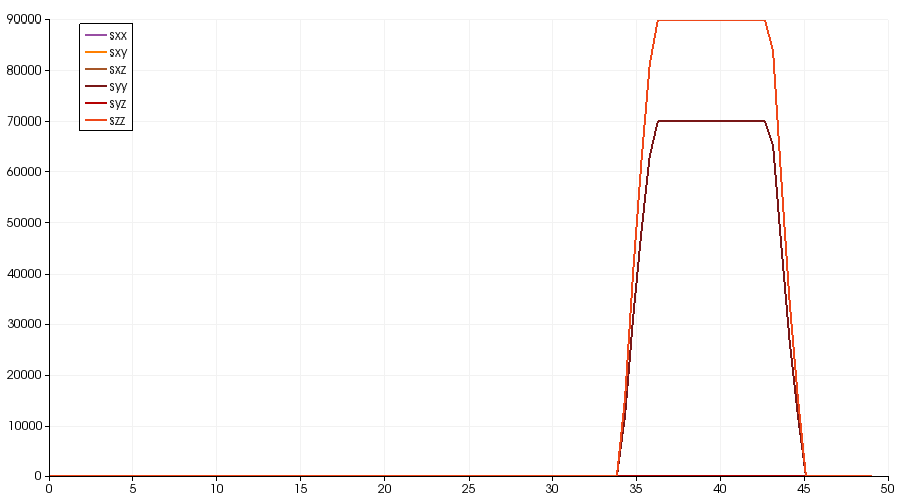
\includegraphics[width=0.8\textwidth]{png/p-wave-test/s/0001.png}
\caption{Распространение P-волны, 1-й временной слой. Изображены компоненты тензора напряжений.}
\label{pic:p_wave_1}
\end{figure}

\begin{figure}[htp]
\centering
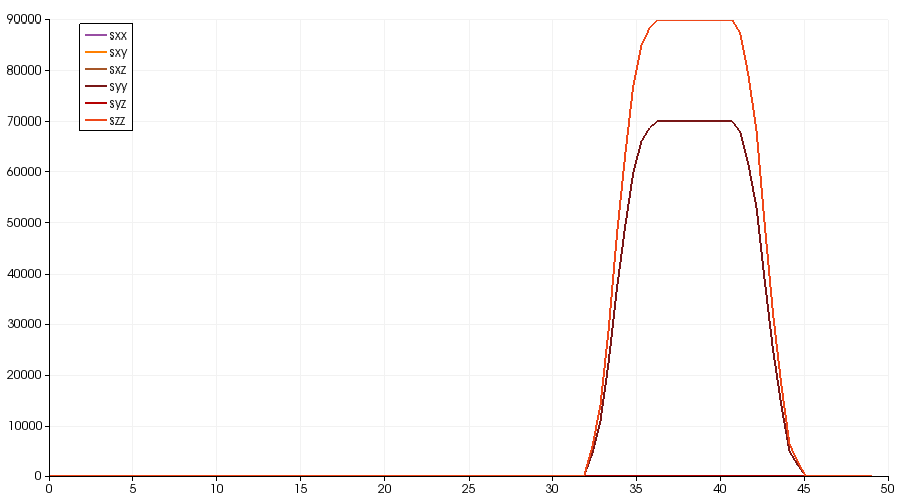
\includegraphics[width=0.8\textwidth]{png/p-wave-test/s/0003.png}
\caption{Распространение P-волны, 3-й временной слой. Изображены компоненты тензора напряжений.}
\end{figure}

\begin{figure}[htp]
\centering
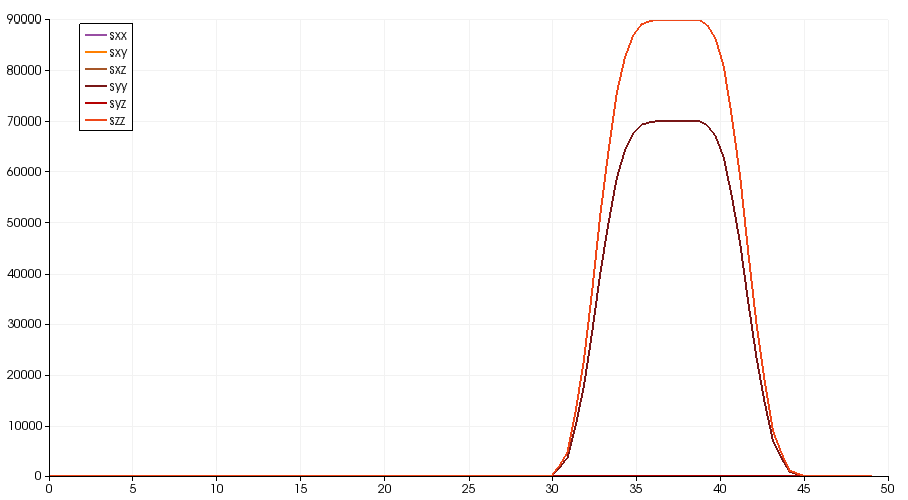
\includegraphics[width=0.8\textwidth]{png/p-wave-test/s/0005.png}
\caption{Распространение P-волны, 5-й временной слой. Изображены компоненты тензора напряжений.}
\end{figure}

\begin{figure}[htp]
\centering
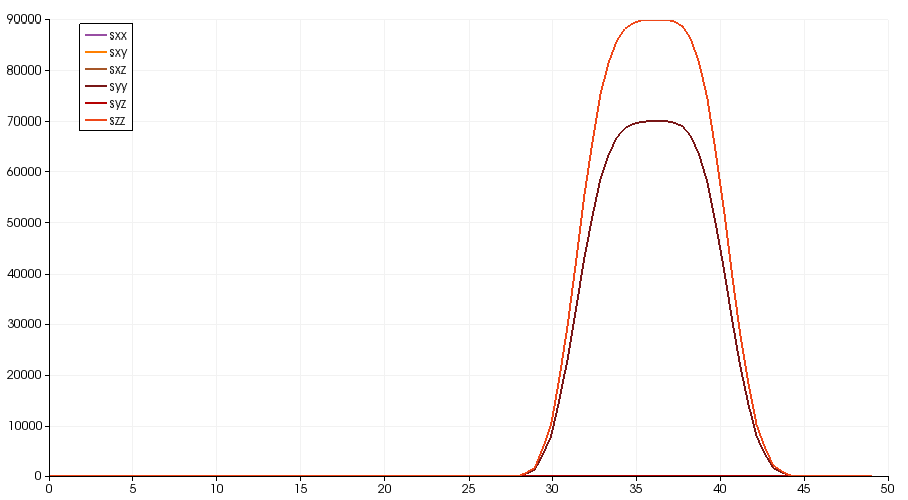
\includegraphics[width=0.8\textwidth]{png/p-wave-test/s/0007.png}
\caption{Распространение P-волны, 7-й временной слой. Изображены компоненты тензора напряжений.}
\end{figure}

\begin{figure}[htp]
\centering
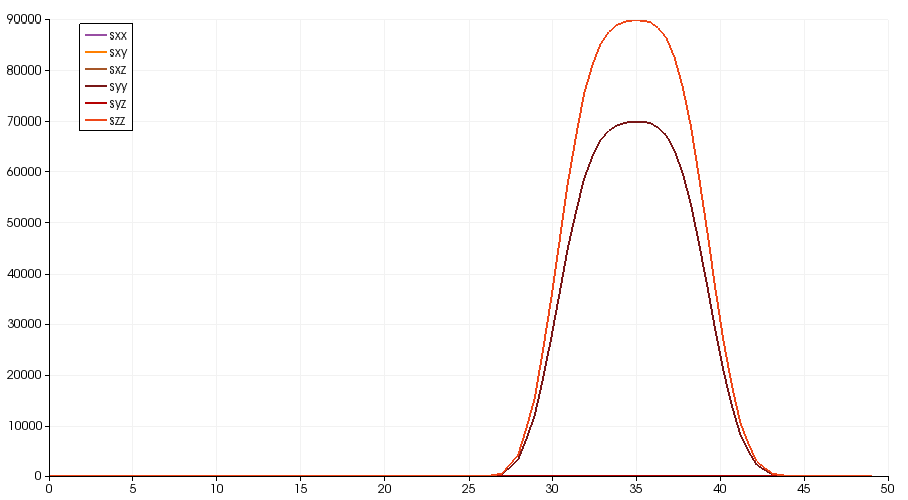
\includegraphics[width=0.8\textwidth]{png/p-wave-test/s/0009.png}
\caption{Распространение P-волны, 9-й временной слой. Изображены компоненты тензора напряжений.}
\end{figure}

\begin{figure}[htp]
\centering
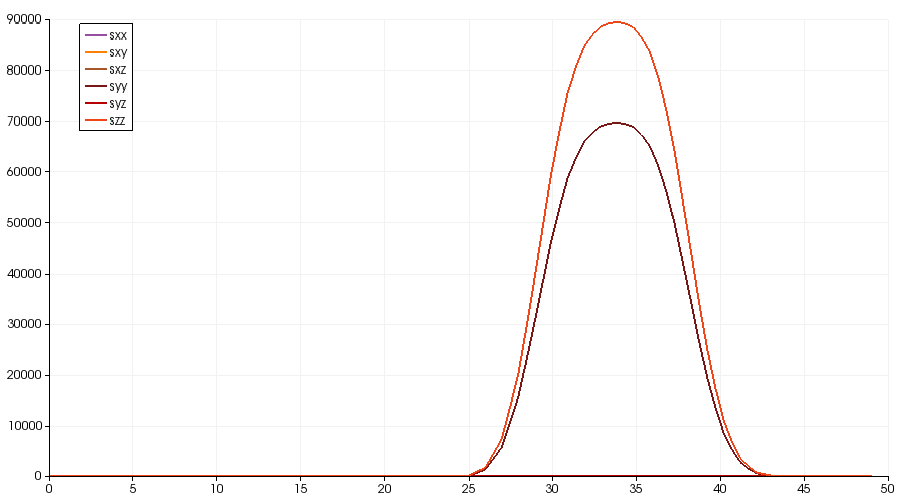
\includegraphics[width=0.8\textwidth]{png/p-wave-test/s/0011.png}
\caption{Распространение P-волны, 11-й временной слой. Изображены компоненты тензора напряжений.}
\end{figure}

\begin{figure}[htp]
\centering
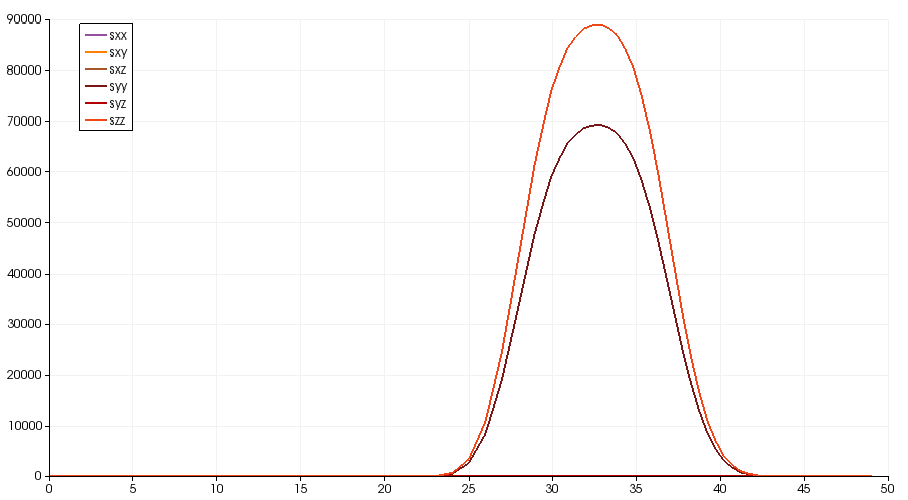
\includegraphics[width=0.8\textwidth]{png/p-wave-test/s/0013.png}
\caption{Распространение P-волны, 13-й временной слой. Изображены компоненты тензора напряжений.}
\end{figure}

\begin{figure}[htp]
\centering
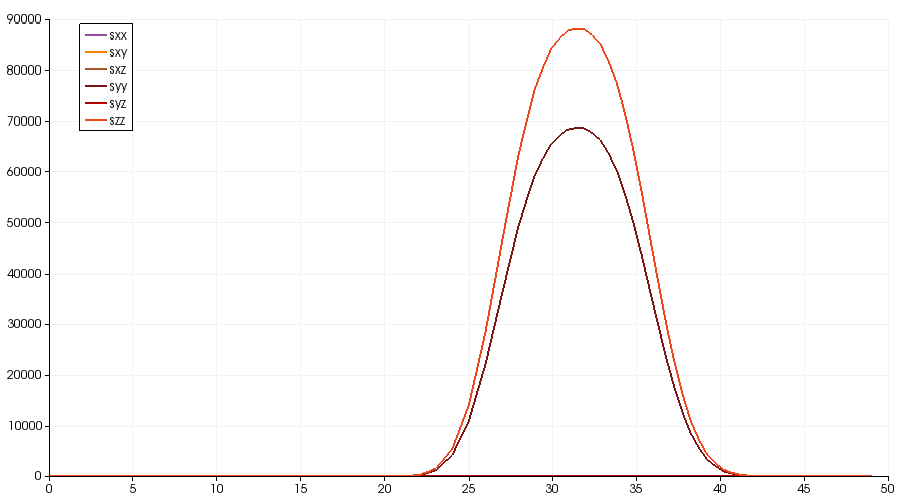
\includegraphics[width=0.8\textwidth]{png/p-wave-test/s/0015.png}
\caption{Распространение P-волны, 15-й временной слой. Изображены компоненты тензора напряжений.}
\label{pic:p_wave_15}
\end{figure}

\clearpage
\newpage

\subsection{Распространение поперечной волны (S-волны)}
Пусть плоская S-волна в среде распространяется вдоль оси z. В этом случае аналитическое решение соответствующего одномерного уравнения дает следующие соотношения на параметры волны:
\begin{itemize}
\item $v_z=-f(z)\sqrt{\frac{\mu}{\rho}}=C_s$;
\item $v_x=v_y=0$;
\item $\sigma_{ij}=f(z)\mu$; для одной из пар $i \neq j$
\item $\sigma_{ij}=0$ для $i = j$.
\end{itemize}
Здесь $f(z)$ - произвольная функция, зависящая только от z и задающая форму волны.
Для расчёта распространения S-волны в кубе были использованы следующие безразмерные параметры: 
\begin{itemize}
\item размер расчётной области: 50x50x50;
\item $\lambda=70000$;
\item $\mu=10000$;
\item $\rho=1$.
\end{itemize}
На графиках (см. рис.
\ref{pic:s_wave_1}-\ref{pic:s_wave_15}) представлены результаты численного расчёта. Получено совпадение скорости волны с аналитическим решением:
\begin{itemize}
\item $v_z=C_s=100$.
\end{itemize}

\begin{figure}[htp]
\centering
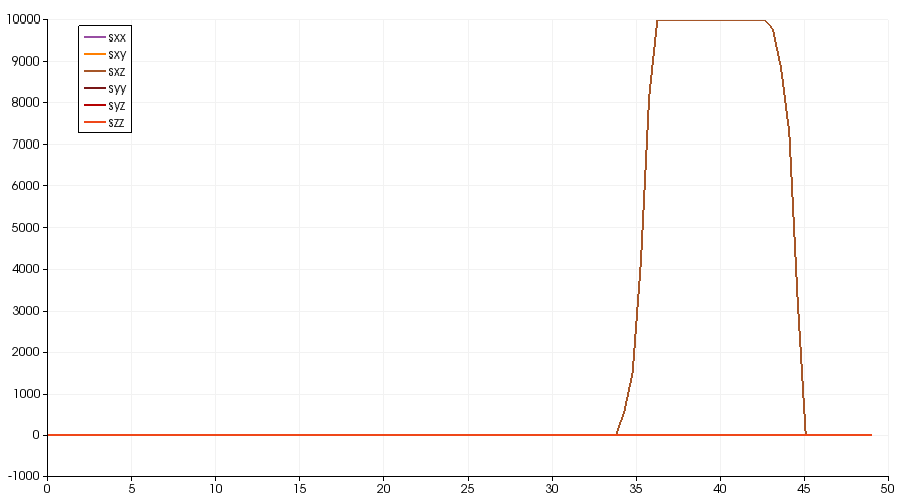
\includegraphics[width=0.8\textwidth]{png/s-wave-test/s/0001.png}
\caption{Распространение S-волны, 1-й временной слой. Изображены компоненты тензора напряжений.}
\label{pic:s_wave_1}
\end{figure}

\begin{figure}[htp]
\centering
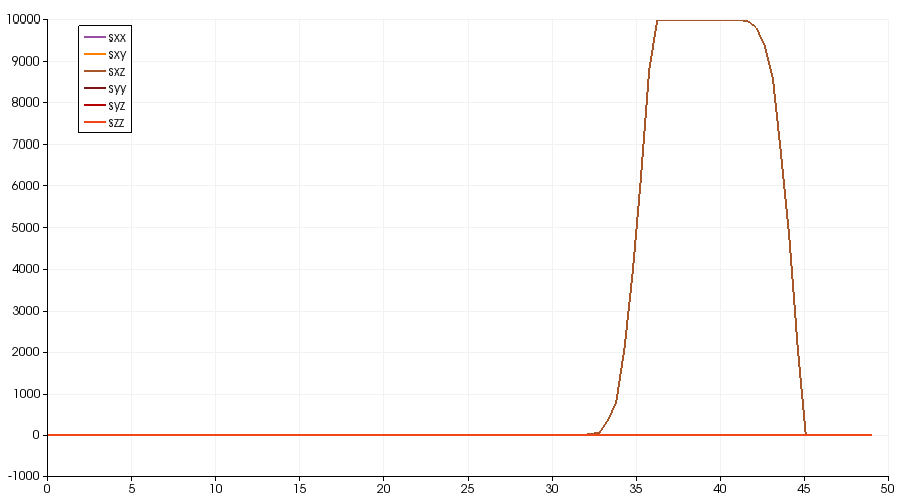
\includegraphics[width=0.8\textwidth]{png/s-wave-test/s/0003.png}
\caption{Распространение S-волны, 3-й временной слой. Изображены компоненты тензора напряжений.}
\end{figure}

\begin{figure}[htp]
\centering
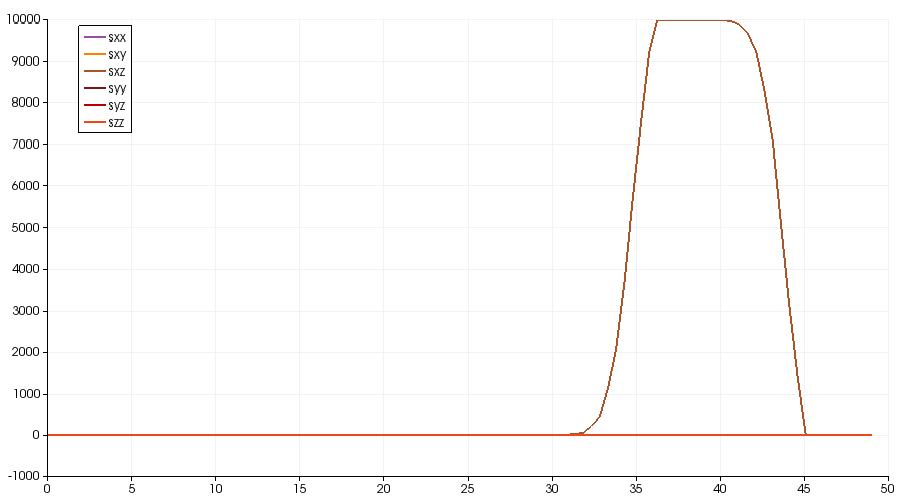
\includegraphics[width=0.8\textwidth]{png/s-wave-test/s/0005.png}
\caption{Распространение S-волны, 5-й временной слой. Изображены компоненты тензора напряжений.}
\end{figure}

\begin{figure}[htp]
\centering
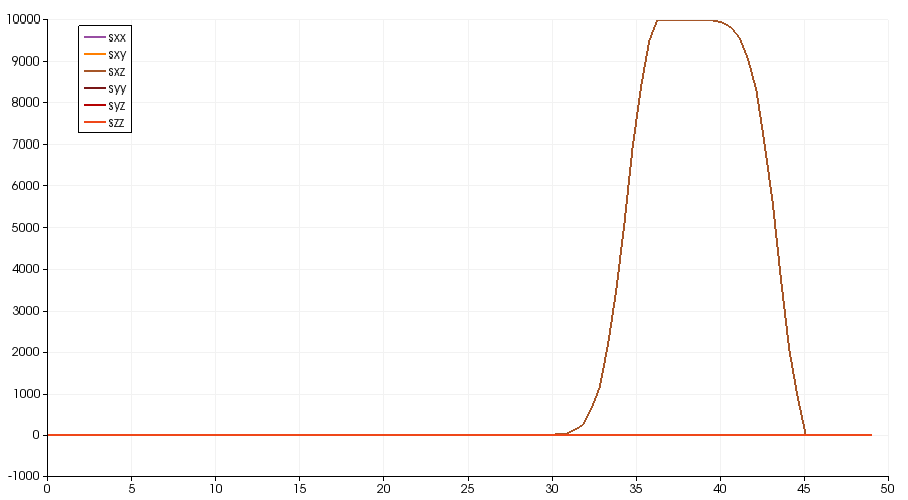
\includegraphics[width=0.8\textwidth]{png/s-wave-test/s/0007.png}
\caption{Распространение S-волны, 7-й временной слой. Изображены компоненты тензора напряжений.}
\end{figure}

\begin{figure}[htp]
\centering
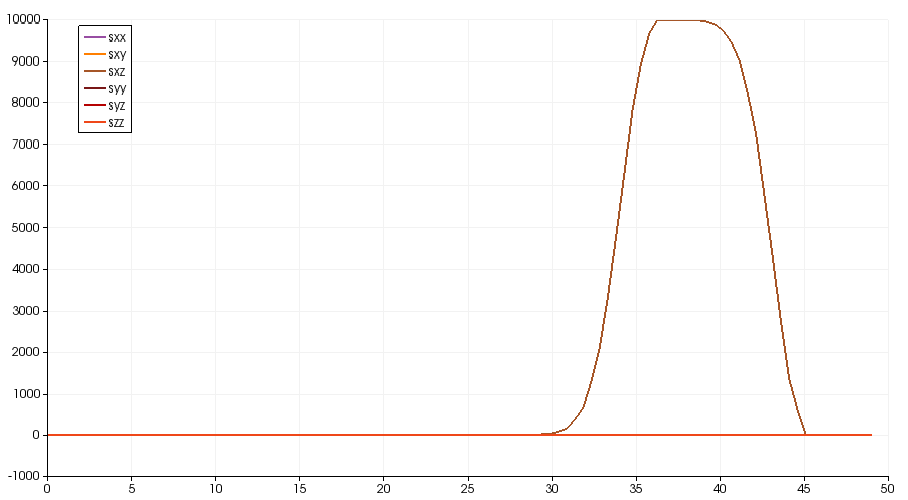
\includegraphics[width=0.8\textwidth]{png/s-wave-test/s/0009.png}
\caption{Распространение S-волны, 9-й временной слой. Изображены компоненты тензора напряжений.}
\end{figure}

\begin{figure}[htp]
\centering
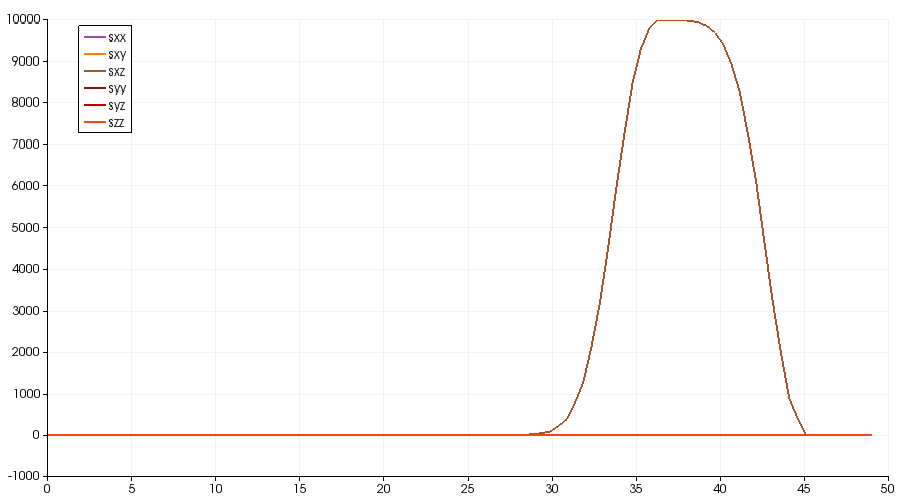
\includegraphics[width=0.8\textwidth]{png/s-wave-test/s/0011.png}
\caption{Распространение S-волны, 11-й временной слой. Изображены компоненты тензора напряжений.}
\end{figure}

\begin{figure}[htp]
\centering
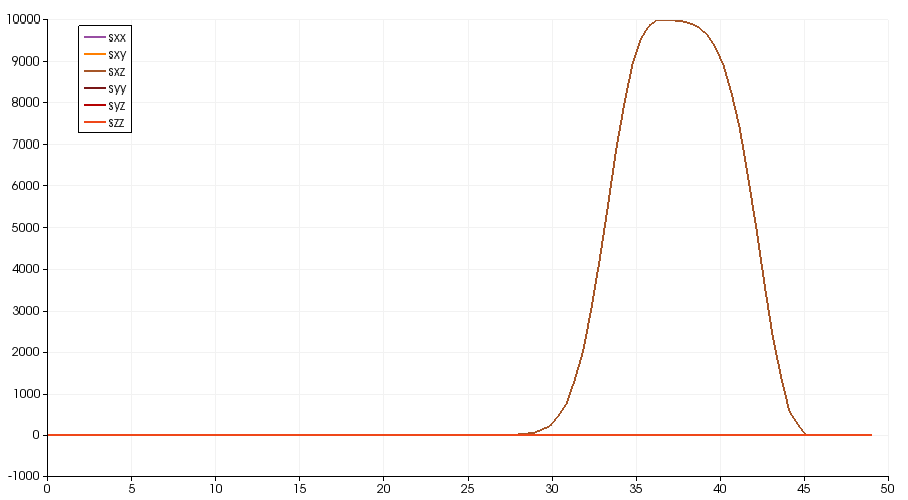
\includegraphics[width=0.8\textwidth]{png/s-wave-test/s/0013.png}
\caption{Распространение S-волны, 13-й временной слой. Изображены компоненты тензора напряжений.}
\end{figure}

\begin{figure}[htp]
\centering
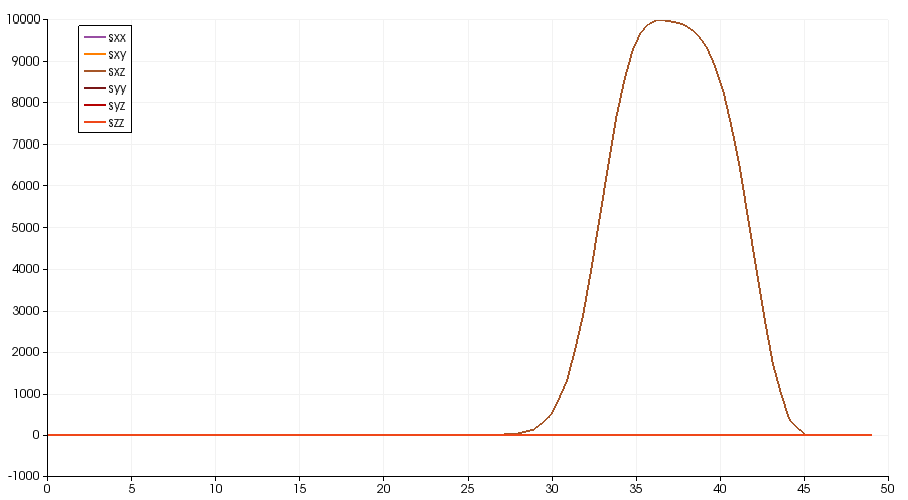
\includegraphics[width=0.8\textwidth]{png/s-wave-test/s/0015.png}
\caption{Распространение S-волны, 15-й временной слой. Изображены компоненты тензора напряжений.}
\label{pic:s_wave_15}
\end{figure}

\clearpage
\newpage

\subsection{Сферический взрыв}
Для проверки изотропии схемы и корректности расчёта при отражении от границ был произведён расчёт
модельной задачи о сферическом взрыве со следующими параметрами:
\begin{itemize}
\item размер расчётной области: 50x50x50;
\item $\lambda=70000$;
\item $\mu=10000$;
\item $\rho=1$.
\end{itemize}
На графиках (см. рис. \ref{pic:spherical_1}-\ref{pic:spherical_70}) изображены
результаты расчётов.

\begin{figure}[htp]
\centering
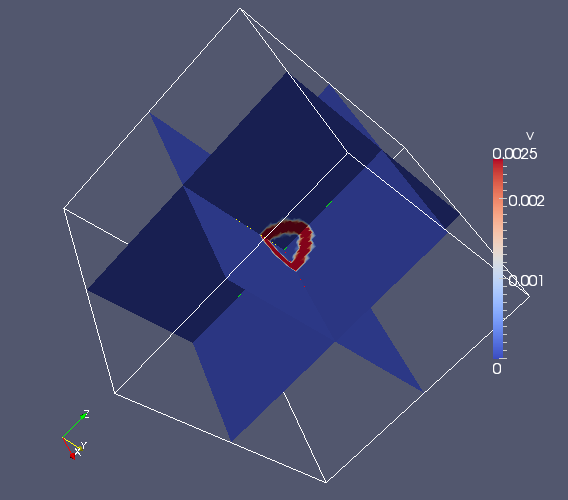
\includegraphics[width=0.6\textwidth]{png/spherical-explosion-test/v-scalar/0001.png}
\caption{Расчёт задачи о сферическом врзыве, 1-й временной слой. Цветом изображен модуль скоростей.}
\label{pic:spherical_1}
\end{figure}

\begin{figure}[htp]
\centering
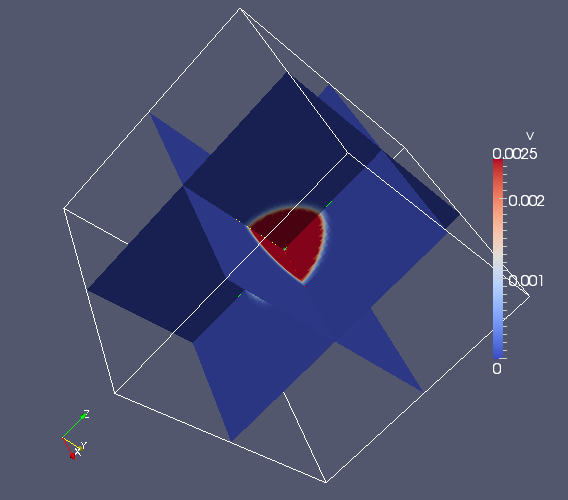
\includegraphics[width=0.6\textwidth]{png/spherical-explosion-test/v-scalar/0005.png}
\caption{Расчёт задачи о сферическом врзыве, 5-й временной слой. Цветом изображен модуль скоростей.}
\end{figure}

\begin{figure}[htp]
\centering
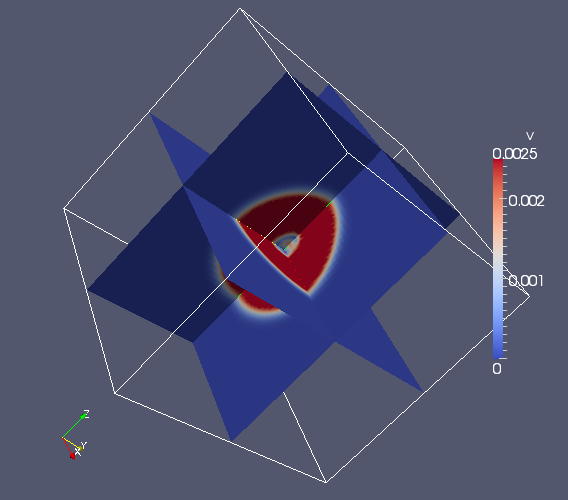
\includegraphics[width=0.6\textwidth]{png/spherical-explosion-test/v-scalar/0010.png}
\caption{Расчёт задачи о сферическом врзыве, 10-й временной слой. Цветом изображен модуль скоростей.}
\end{figure}

\begin{figure}[htp]
\centering
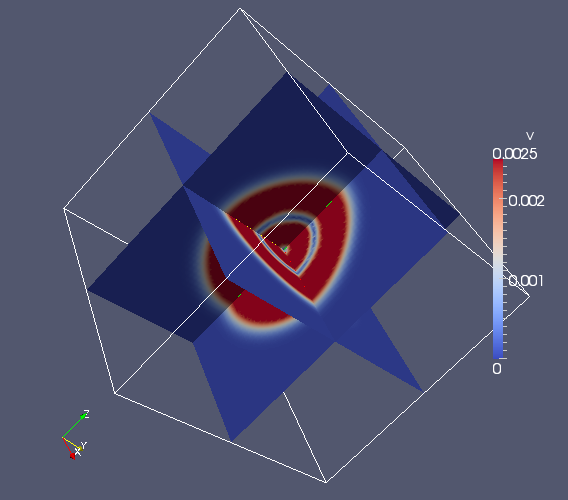
\includegraphics[width=0.6\textwidth]{png/spherical-explosion-test/v-scalar/0015.png}
\caption{Расчёт задачи о сферическом врзыве, 15-й временной слой. Цветом изображен модуль скоростей.}
\end{figure}

\begin{figure}[htp]
\centering
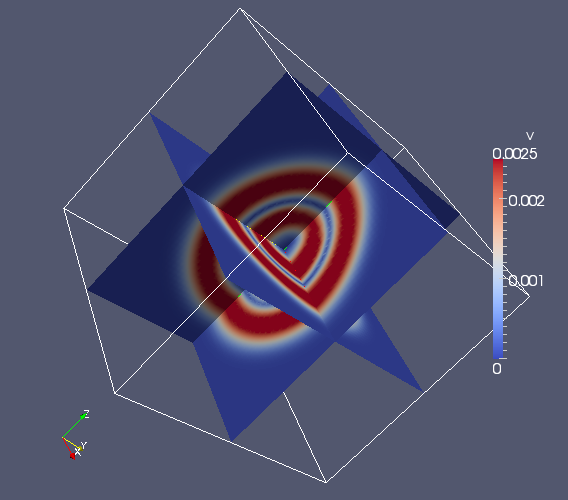
\includegraphics[width=0.6\textwidth]{png/spherical-explosion-test/v-scalar/0020.png}
\caption{Расчёт задачи о сферическом врзыве, 20-й временной слой. Цветом изображен модуль скоростей.}
\end{figure}

\begin{figure}[htp]
\centering
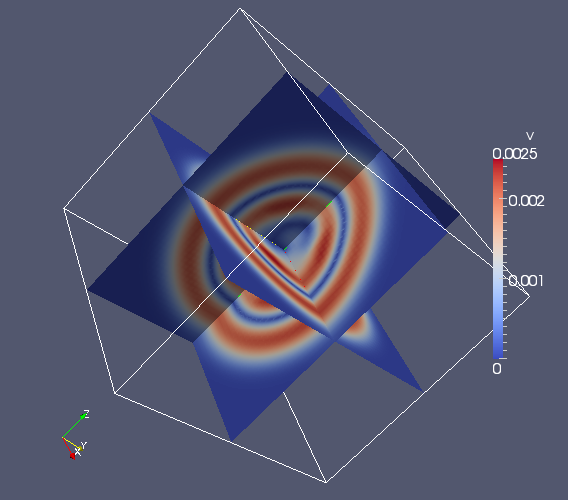
\includegraphics[width=0.6\textwidth]{png/spherical-explosion-test/v-scalar/0025.png}
\caption{Расчёт задачи о сферическом врзыве, 25-й временной слой. Цветом изображен модуль скоростей.}
\end{figure}

\begin{figure}[htp]
\centering
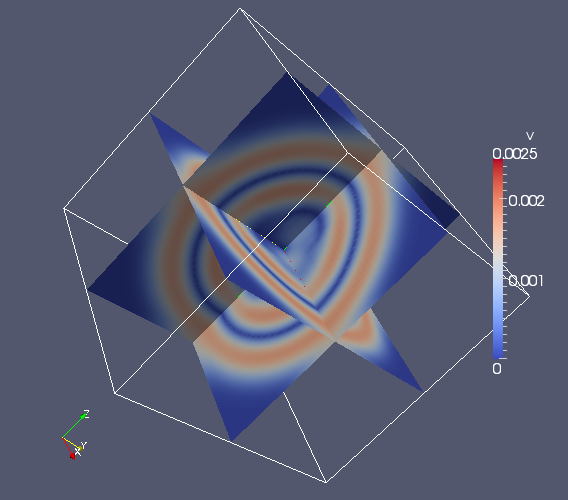
\includegraphics[width=0.6\textwidth]{png/spherical-explosion-test/v-scalar/0030.png}
\caption{Расчёт задачи о сферическом врзыве, 30-й временной слой. Цветом изображен модуль скоростей.}
\end{figure}

\begin{figure}[htp]
\centering
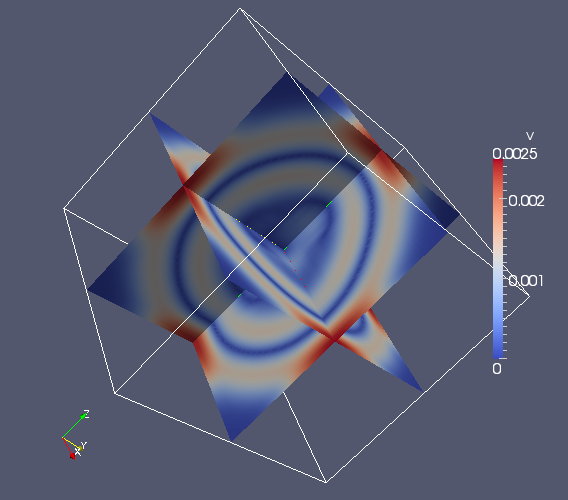
\includegraphics[width=0.6\textwidth]{png/spherical-explosion-test/v-scalar/0035.png}
\caption{Расчёт задачи о сферическом врзыве, 35-й временной слой. Цветом изображен модуль скоростей.}
\end{figure}

\begin{figure}[htp]
\centering
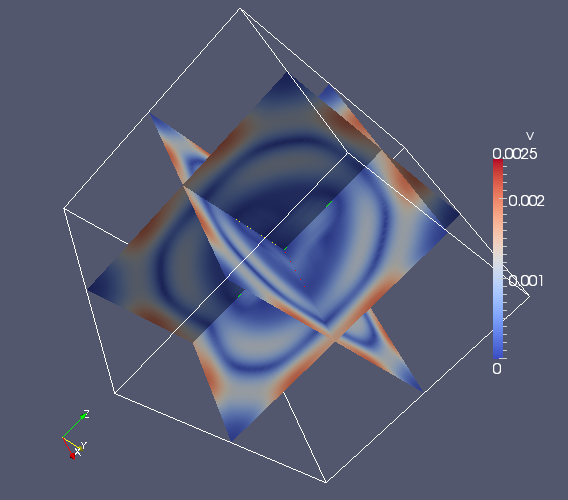
\includegraphics[width=0.6\textwidth]{png/spherical-explosion-test/v-scalar/0040.png}
\caption{Расчёт задачи о сферическом врзыве, 40-й временной слой. Цветом изображен модуль скоростей.}
\end{figure}

\begin{figure}[htp]
\centering
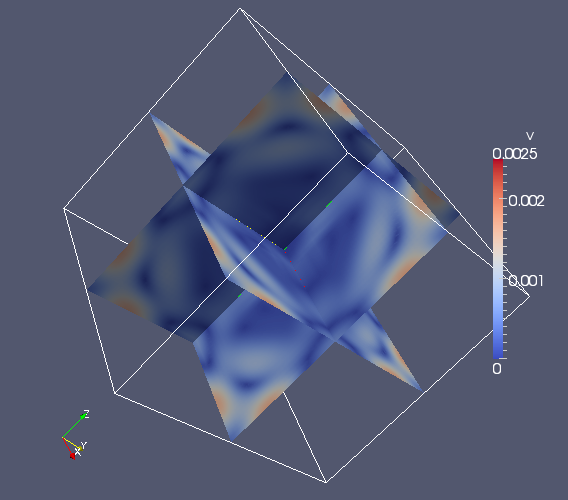
\includegraphics[width=0.6\textwidth]{png/spherical-explosion-test/v-scalar/0045.png}
\caption{Расчёт задачи о сферическом врзыве, 45-й временной слой. Цветом изображен модуль скоростей.}
\end{figure}

\begin{figure}[htp]
\centering
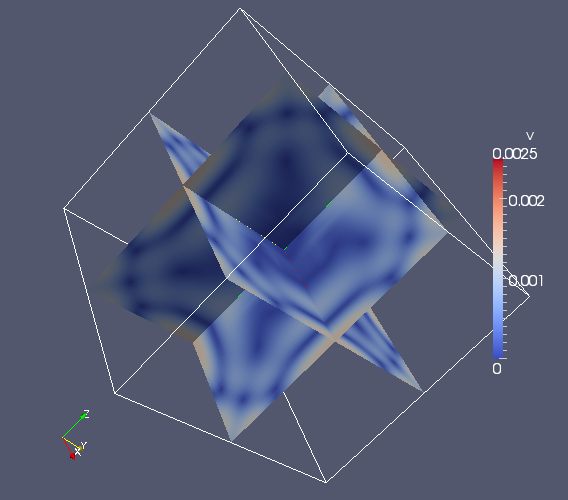
\includegraphics[width=0.6\textwidth]{png/spherical-explosion-test/v-scalar/0050.png}
\caption{Расчёт задачи о сферическом врзыве, 50-й временной слой. Цветом изображен модуль скоростей.}
\end{figure}

\begin{figure}[htp]
\centering
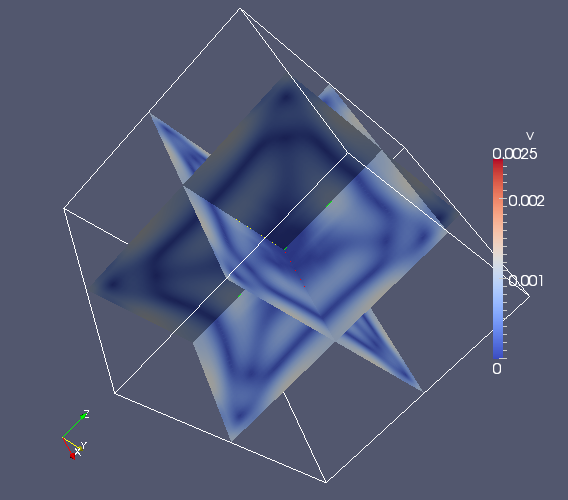
\includegraphics[width=0.6\textwidth]{png/spherical-explosion-test/v-scalar/0055.png}
\caption{Расчёт задачи о сферическом врзыве, 55-й временной слой. Цветом изображен модуль скоростей.}
\end{figure}

\begin{figure}[htp]
\centering
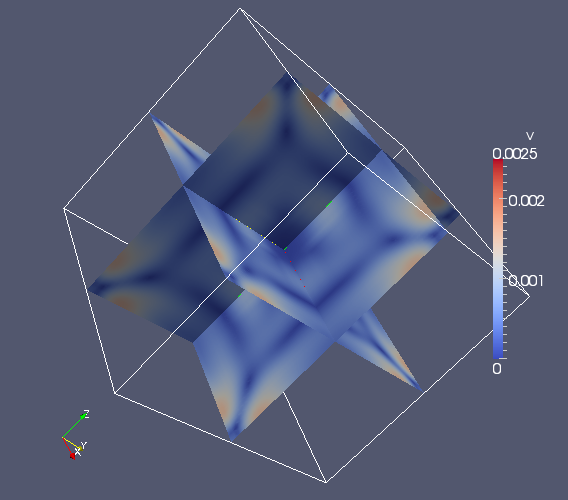
\includegraphics[width=0.6\textwidth]{png/spherical-explosion-test/v-scalar/0060.png}
\caption{Расчёт задачи о сферическом врзыве, 60-й временной слой. Цветом изображен модуль скоростей.}
\end{figure}

\begin{figure}[htp]
\centering
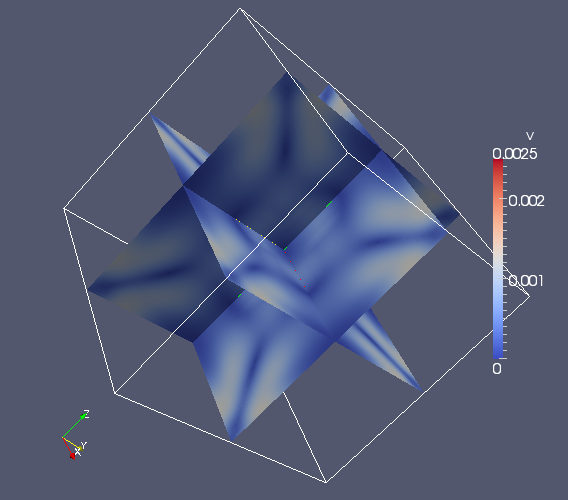
\includegraphics[width=0.6\textwidth]{png/spherical-explosion-test/v-scalar/0065.png}
\caption{Расчёт задачи о сферическом врзыве, 65-й временной слой. Цветом изображен модуль скоростей.}
\end{figure}

\begin{figure}[htp]
\centering
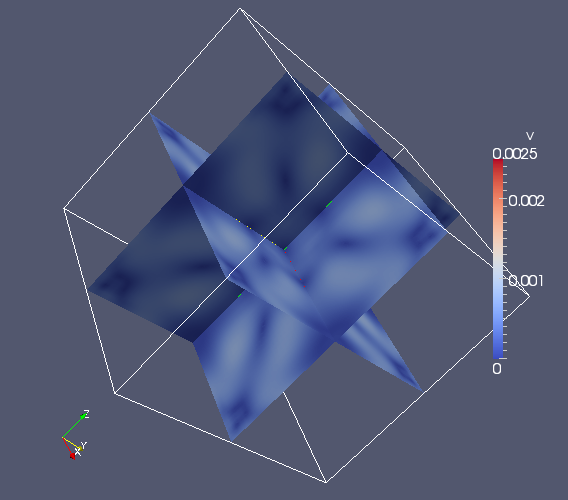
\includegraphics[width=0.6\textwidth]{png/spherical-explosion-test/v-scalar/0070.png}
\caption{Расчёт задачи о сферическом врзыве, 70-й временной слой. Цветом изображен модуль скоростей.}
\label{pic:spherical_70}
\end{figure}

\clearpage
\newpage

\subsection{Конечные деформации}
Для проверки расчета при конечных деформациях был выполнен расчёт модельной задачи о воздействии ударника на пластину. Воздействие задавалось граничным условием на нормальную компоненту силы в области удара.

На графиках (см. рис. \ref{pic:moving_border_1}-\ref{pic:moving_border_40}) изображены результаты расчётов.

\begin{figure}[htp]
\centering
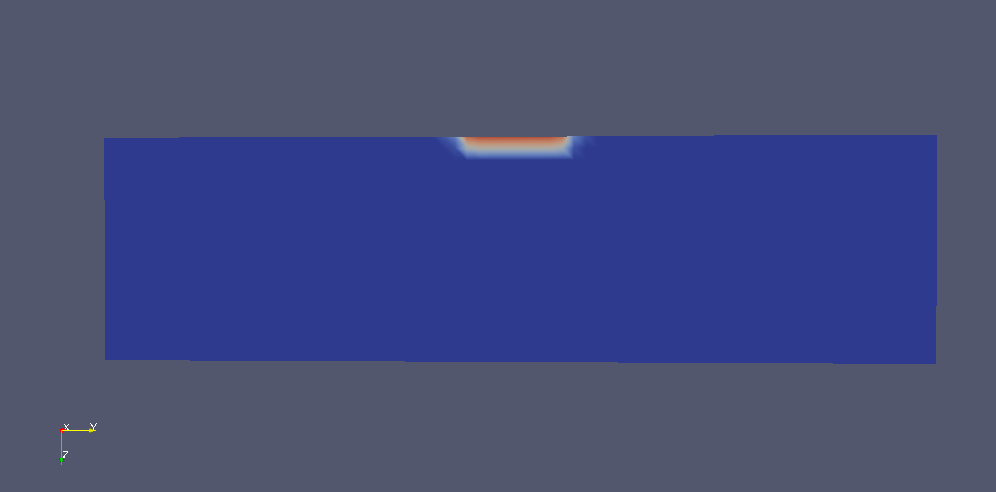
\includegraphics[width=0.6\textwidth]{png/border-test/v-2d/0001.png}
\caption{Расчёт задачи о вхождении ударника в пластину, 1-й временной слой. Цветом изображен модуль скоростей.}
\label{pic:moving_border_1}
\end{figure}

\begin{figure}[htp]
\centering
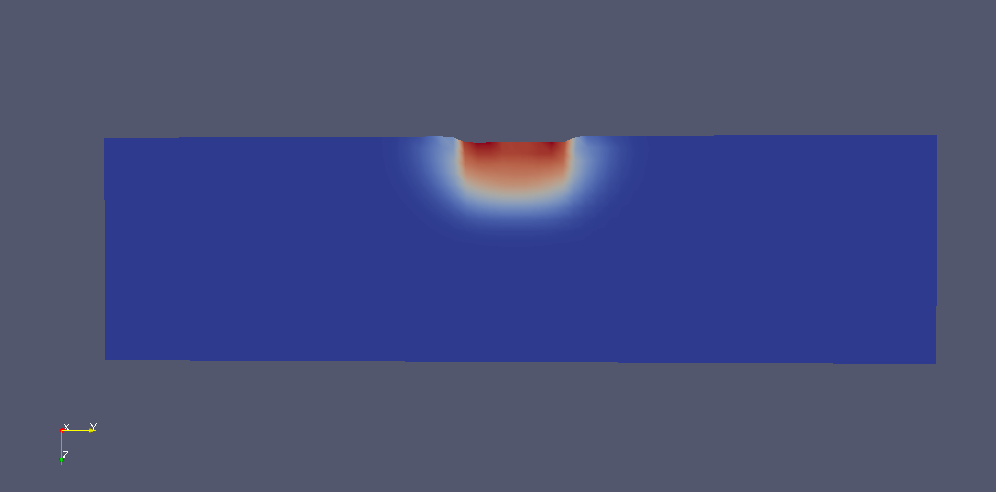
\includegraphics[width=0.6\textwidth]{png/border-test/v-2d/0010.png}
\caption{Расчёт задачи о вхождении ударника в пластину, 10-й временной слой. Цветом изображен модуль скоростей.}
\end{figure}

\begin{figure}[htp]
\centering
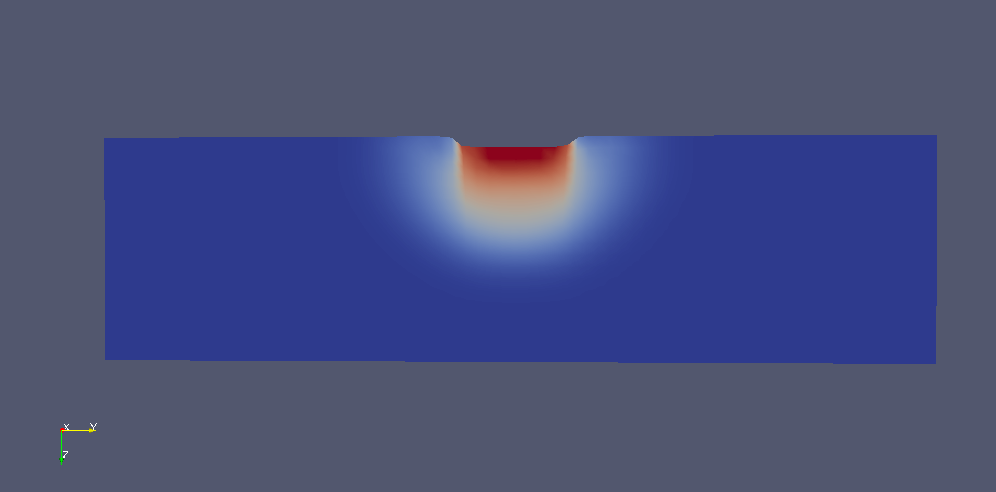
\includegraphics[width=0.6\textwidth]{png/border-test/v-2d/0020.png}
\caption{Расчёт задачи о вхождении ударника в пластину, 20-й временной слой. Цветом изображен модуль скоростей.}
\end{figure}

\begin{figure}[htp]
\centering
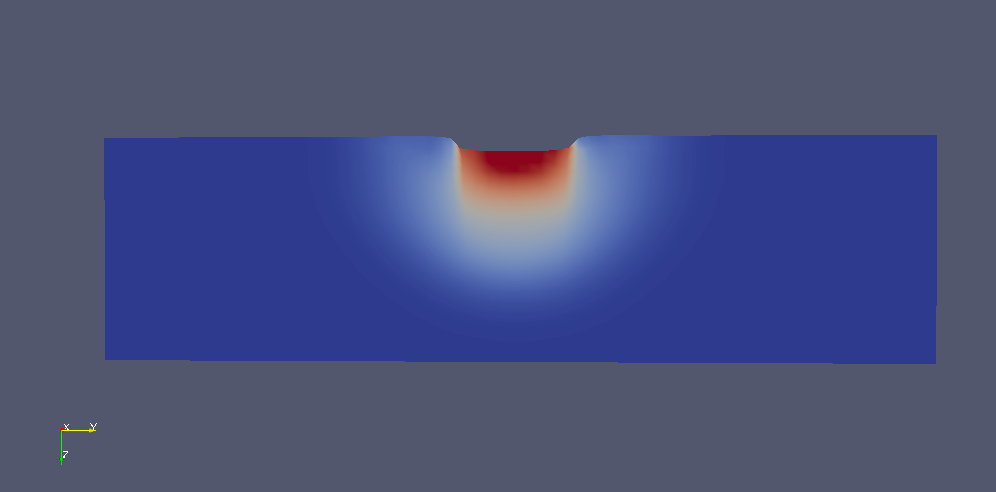
\includegraphics[width=0.6\textwidth]{png/border-test/v-2d/0030.png}
\caption{Расчёт задачи о вхождении ударника в пластину, 30-й временной слой. Цветом изображен модуль скоростей.}
\end{figure}

\begin{figure}[htp]
\centering
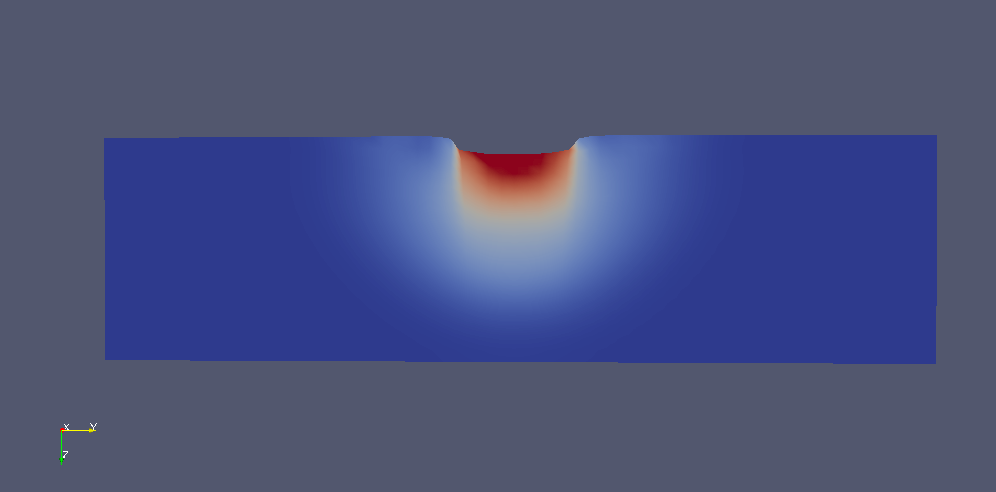
\includegraphics[width=0.6\textwidth]{png/border-test/v-2d/0040.png}
\caption{Расчёт задачи о вхождении ударника в пластину, 40-й временной слой. Цветом изображен модуль скоростей.}
\label{pic:moving_border_40}
\end{figure}


\clearpage
\newpage

\subsection{Контакт тел}
Для проверки расчета контактных границ и взаимодействия тел был выполнен расчёт задачи об ударе по пластине с явным моделированием пластины и ударника на отдельных сетках.

На графиках (см. рис. \ref{pic:striker_test_2d_1}-\ref{pic:striker_test_2d_280}) изображены поля скоростей в пластине и ударнике.

\begin{figure}[htp]
\centering
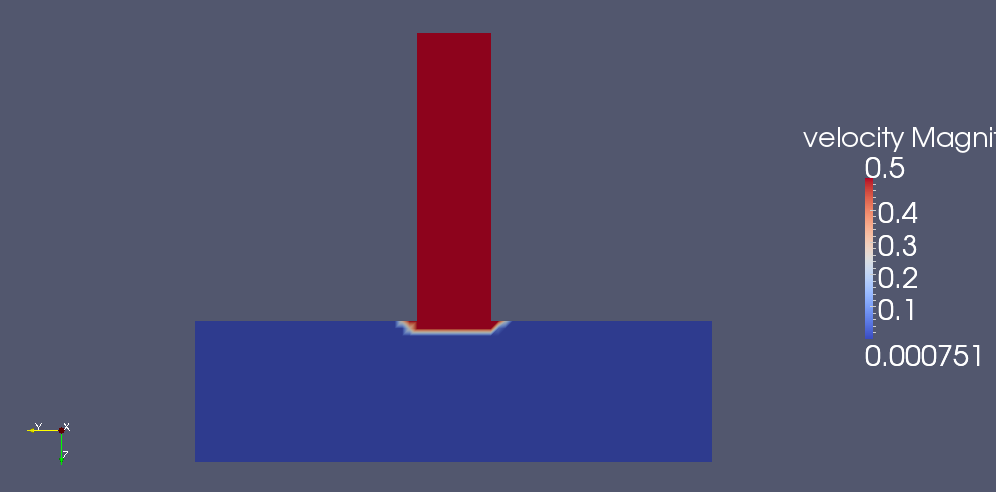
\includegraphics[width=0.6\textwidth]{png/strike-test/both-2d/0001.png}
\caption{Поля скоростей в ударнике и пластине. 1-й временной слой. Цветом изображен модуль скорости.}
\label{pic:striker_test_2d_1}
\end{figure}

\begin{figure}[htp]
\centering
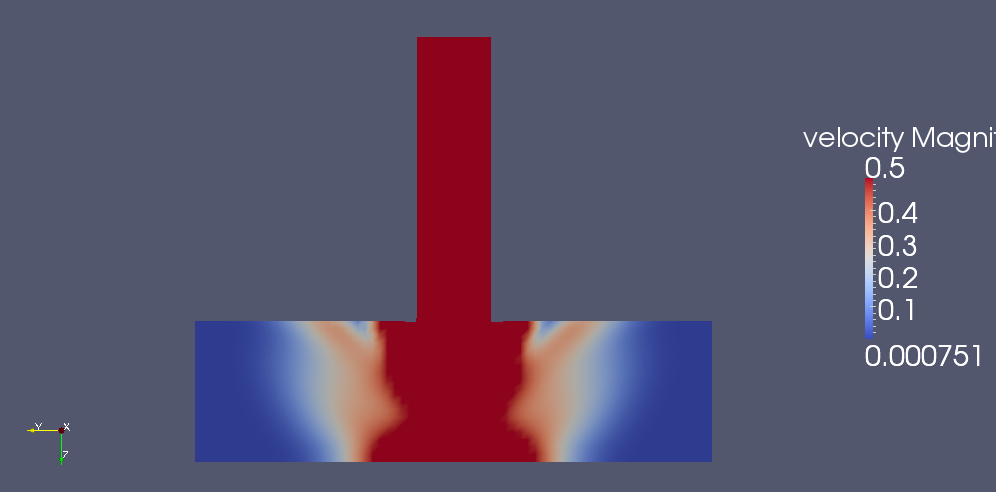
\includegraphics[width=0.6\textwidth]{png/strike-test/both-2d/0040.png}
\caption{Поля скоростей в ударнике и пластине. 40-й временной слой. Цветом изображен модуль скорости.}
\end{figure}

\begin{figure}[htp]
\centering
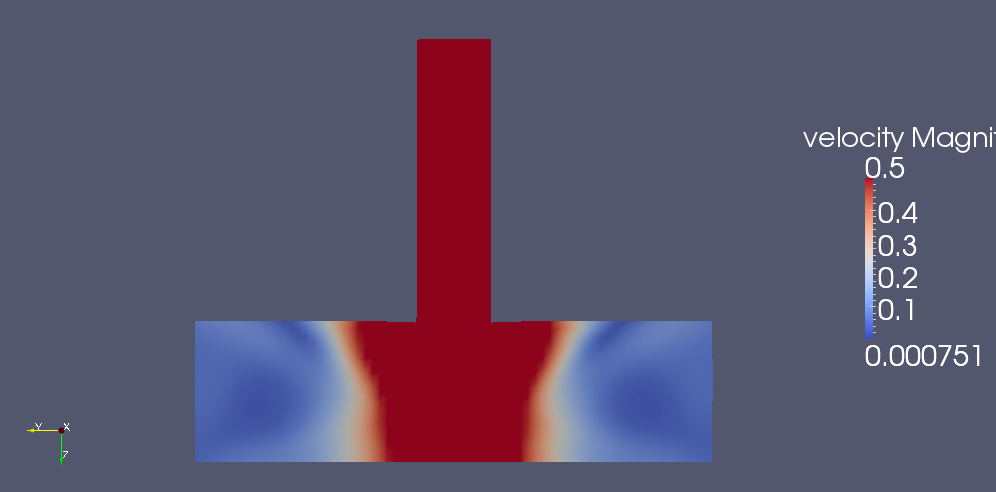
\includegraphics[width=0.6\textwidth]{png/strike-test/both-2d/0080.png}
\caption{Поля скоростей в ударнике и пластине. 80-й временной слой. Цветом изображен модуль скорости.}
\end{figure}

\begin{figure}[htp]
\centering
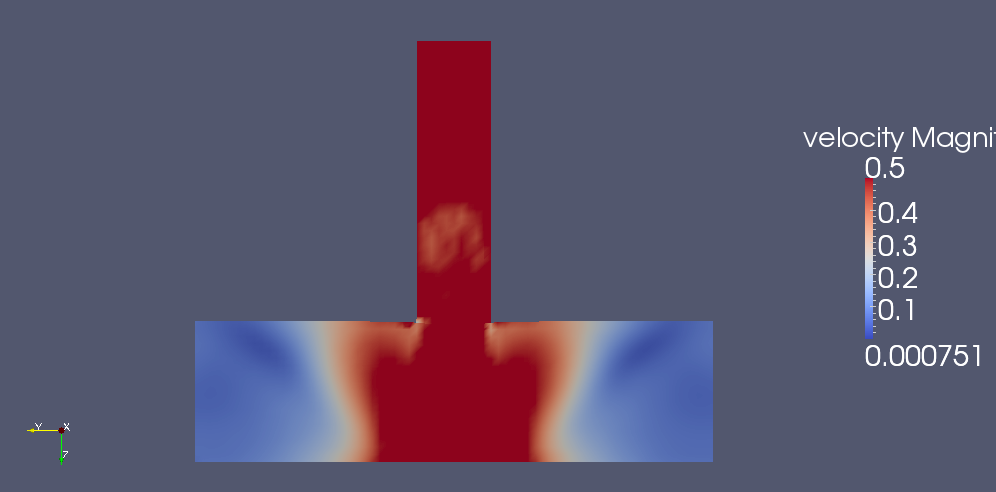
\includegraphics[width=0.6\textwidth]{png/strike-test/both-2d/0120.png}
\caption{Поля скоростей в ударнике и пластине. 120-й временной слой. Цветом изображен модуль скорости.}
\end{figure}

\begin{figure}[htp]
\centering
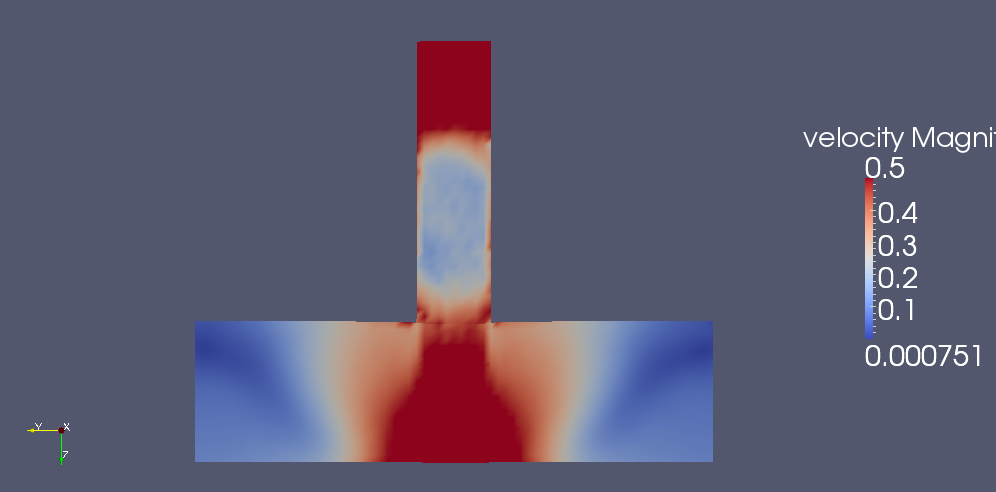
\includegraphics[width=0.6\textwidth]{png/strike-test/both-2d/0160.png}
\caption{Поля скоростей в ударнике и пластине. 160-й временной слой. Цветом изображен модуль скорости.}
\end{figure}

\begin{figure}[htp]
\centering
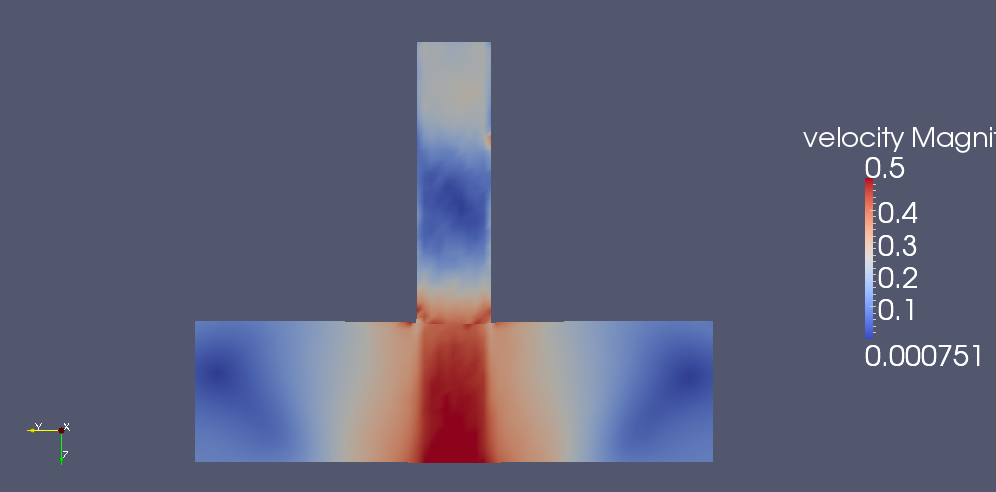
\includegraphics[width=0.6\textwidth]{png/strike-test/both-2d/0200.png}
\caption{Поля скоростей в ударнике и пластине. 200-й временной слой. Цветом изображен модуль скорости.}
\end{figure}

\begin{figure}[htp]
\centering
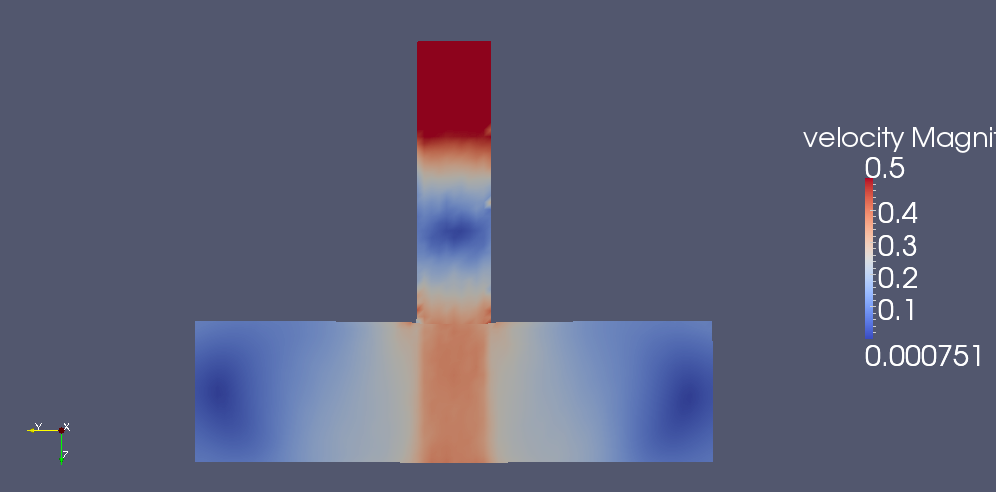
\includegraphics[width=0.6\textwidth]{png/strike-test/both-2d/0240.png}
\caption{Поля скоростей в ударнике и пластине. 240-й временной слой. Цветом изображен модуль скорости.}
\end{figure}

\begin{figure}[htp]
\centering
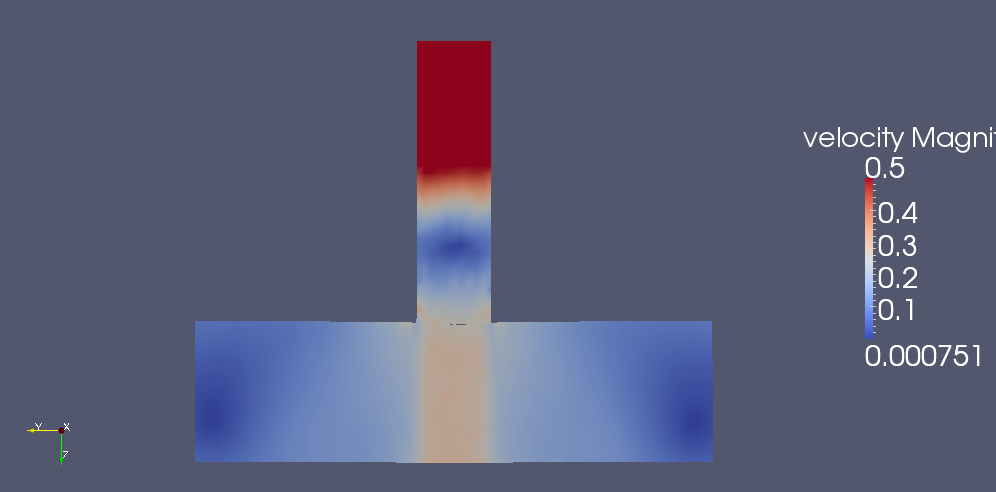
\includegraphics[width=0.6\textwidth]{png/strike-test/both-2d/0280.png}
\caption{Поля скоростей в ударнике и пластине. 280-й временной слой. Цветом изображен модуль скорости.}
\label{pic:striker_test_2d_280}
\end{figure}

\clearpage

На графиках (см. рис. \ref{pic:striker_test_plate_1}-\ref{pic:striker_test_plate_200}) изображено трёхмерное распределение поля скоростей в пластине.

\begin{figure}[htp]
\centering
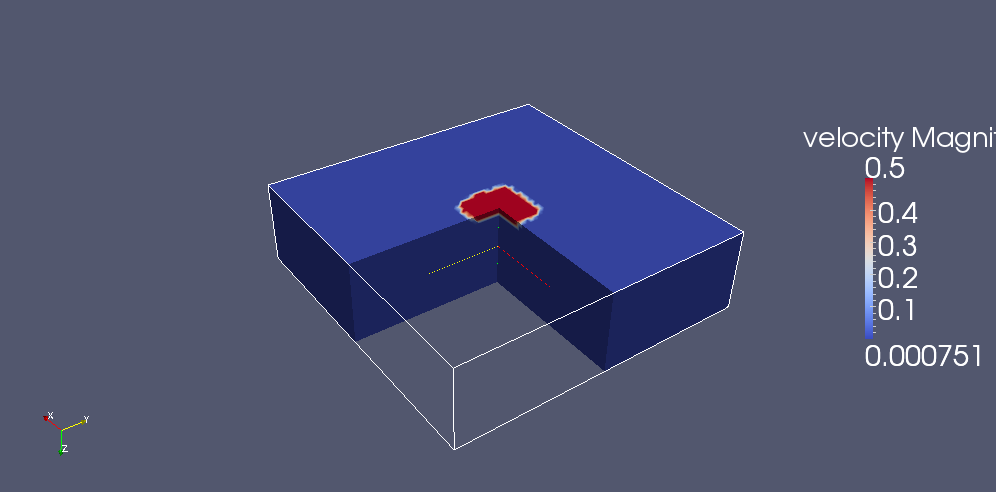
\includegraphics[width=0.6\textwidth]{png/strike-test/plate-3d-v/0001.png}
\caption{Трёхмерное распределение поля скоростей в пластине. 1-й временной слой. Цветом изображен модуль скорости.}
\label{pic:striker_test_plate_1}
\end{figure}

\begin{figure}[htp]
\centering
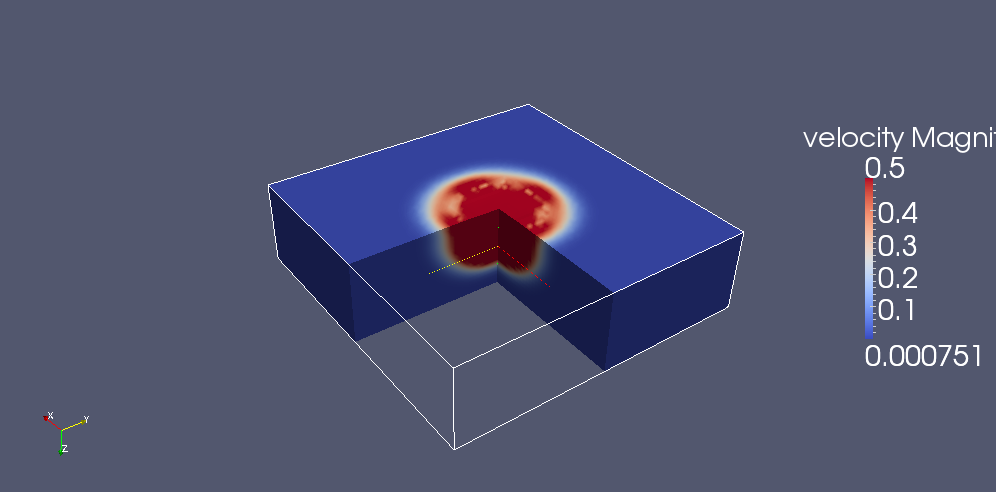
\includegraphics[width=0.6\textwidth]{png/strike-test/plate-3d-v/0020.png}
\caption{Трёхмерное распределение поля скоростей в пластине. 20-й временной слой. Цветом изображен модуль скорости.}
\end{figure}

\begin{figure}[htp]
\centering
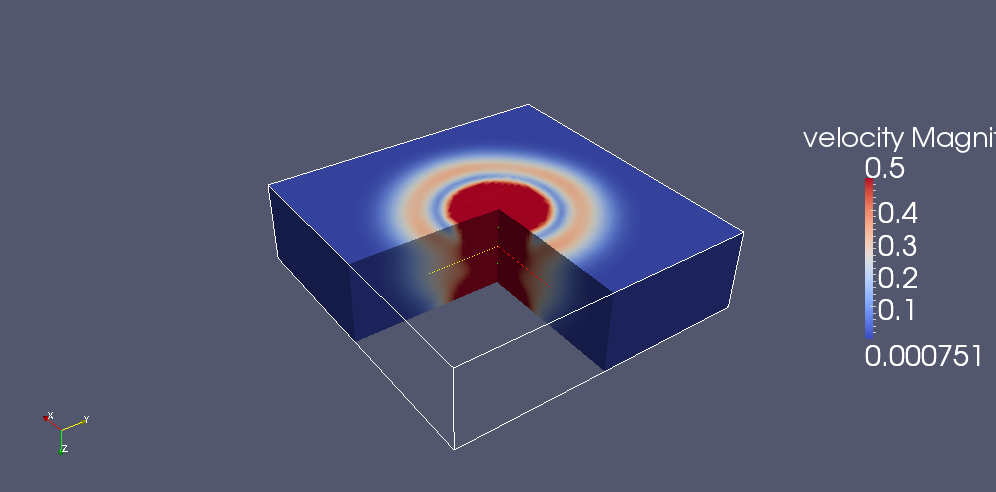
\includegraphics[width=0.6\textwidth]{png/strike-test/plate-3d-v/0040.png}
\caption{Трёхмерное распределение поля скоростей в пластине. 40-й временной слой. Цветом изображен модуль скорости.}
\end{figure}

\begin{figure}[htp]
\centering
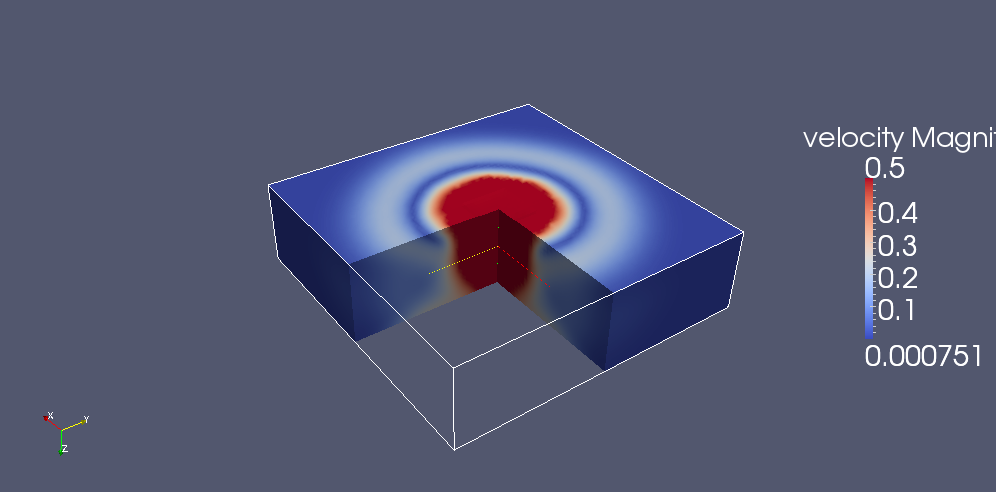
\includegraphics[width=0.6\textwidth]{png/strike-test/plate-3d-v/0060.png}
\caption{Трёхмерное распределение поля скоростей в пластине. 60-й временной слой. Цветом изображен модуль скорости.}
\end{figure}

\begin{figure}[htp]
\centering
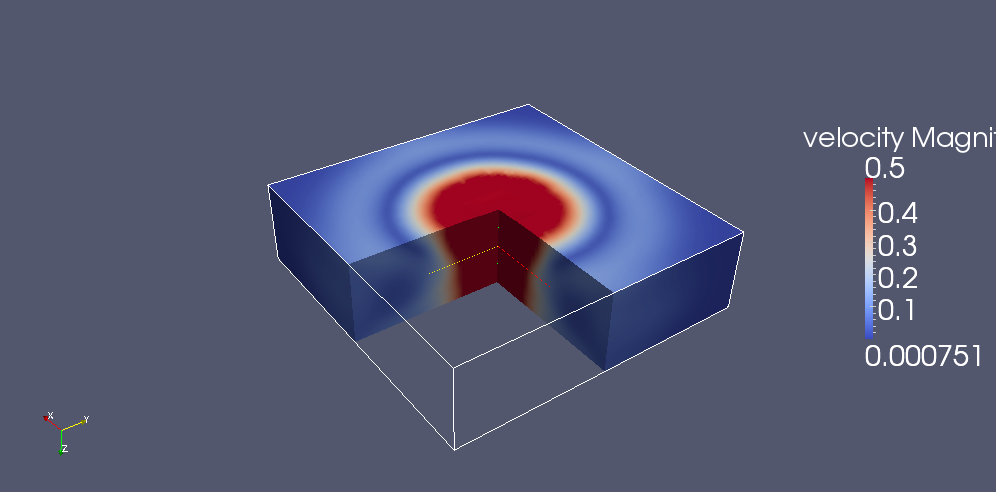
\includegraphics[width=0.6\textwidth]{png/strike-test/plate-3d-v/0080.png}
\caption{Трёхмерное распределение поля скоростей в пластине. 80-й временной слой. Цветом изображен модуль скорости.}
\end{figure}

\begin{figure}[htp]
\centering
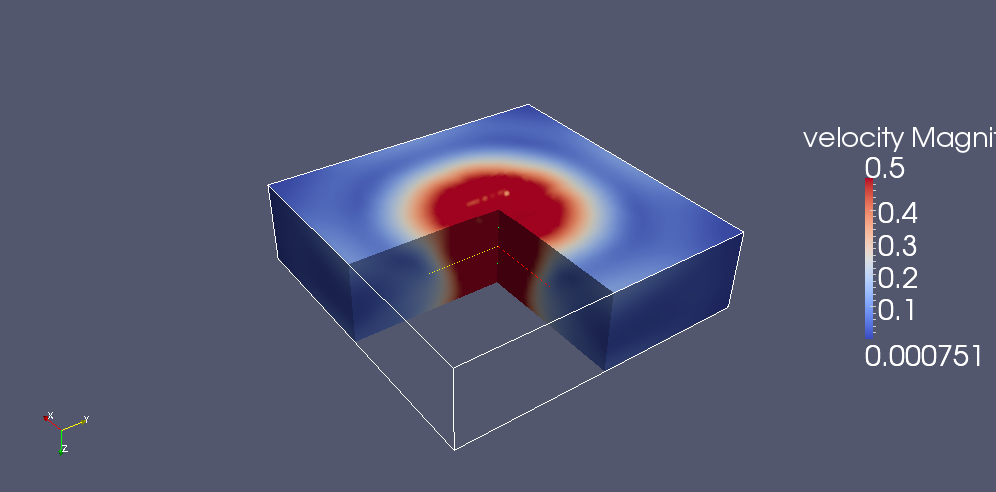
\includegraphics[width=0.6\textwidth]{png/strike-test/plate-3d-v/0100.png}
\caption{Трёхмерное распределение поля скоростей в пластине. 100-й временной слой. Цветом изображен модуль скорости.}
\end{figure}

\begin{figure}[htp]
\centering
\includegraphics[width=0.6\textwidth]{png/strike-test/plate-3d-v/0120.png}
\caption{Трёхмерное распределение поля скоростей в пластине. 120-й временной слой. Цветом изображен модуль скорости.}
\end{figure}

\begin{figure}[htp]
\centering
\includegraphics[width=0.6\textwidth]{png/strike-test/plate-3d-v/0140.png}
\caption{Трёхмерное распределение поля скоростей в пластине. 140-й временной слой. Цветом изображен модуль скорости.}
\end{figure}

\begin{figure}[htp]
\centering
\includegraphics[width=0.6\textwidth]{png/strike-test/plate-3d-v/0160.png}
\caption{Трёхмерное распределение поля скоростей в пластине. 160-й временной слой. Цветом изображен модуль скорости.}
\end{figure}

\begin{figure}[htp]
\centering
\includegraphics[width=0.6\textwidth]{png/strike-test/plate-3d-v/0180.png}
\caption{Трёхмерное распределение поля скоростей в пластине. 180-й временной слой. Цветом изображен модуль скорости.}
\end{figure}

\begin{figure}[htp]
\centering
\includegraphics[width=0.6\textwidth]{png/strike-test/plate-3d-v/0200.png}
\caption{Трёхмерное распределение поля скоростей в пластине. 200-й временной слой. Цветом изображен модуль скорости.}
\label{pic:striker_test_plate_200}
\end{figure}

\clearpage
\newpage

\subsection{Критерии разрушения в однородном материале}

Для тестирования работы критериев разрушения был проведен расчет соударения ударника и монолитной преграды (см. рис. \ref{pic:destruction_test}). Область наибольшей концентрации сжимающих и сдвиговых напряжений локализуется в месте удара и имеет характерные размеры порядка размера ударника. Растягивающие напряжения действуют как в области удара (на этапе отскока), так и в тыльных областях ударника и пластины. Сдвиговые напряжения, помимо области удара, образуют откольный конус с тыльной стороны пластины. Распределение сдвиговых напряжений и напряжения Мизеса качественно совпадают.

\begin{figure}[htp]
\centering
\includegraphics[width=0.45\textwidth]{png/destruction_test.png}
\caption{Тестирование критериев разрушения: а - сжимающие напряжения, б - растягивающие напряжения, в - сдвиговые напряжения, г – приведенные напряжения (критерий Мизеса).}
\label{pic:destruction_test}
\end{figure}

\clearpage
\newpage

\subsection{Волны в многослойной преграде}

При расчёте задачи о непробивающем ударе по многослойной преграде использовались
данные из табл. \ref{tbl:subpackage}. В табл. \ref{tbl:subpackage_2} приведены
безразмерные величины, использовавшиеся в расчёте.
\begin{table}[h]
\centering
\begin{tabular}{|c|c|c|c|}
\hline
Слой & $\rho$ & $\lambda$ & $\mu$  \\
\hline
Эпоксидная смола & 1.25 & 1440 & 960 \\
Субпакет & 1.25 & 4620 & 3080 \\
\hline
\end{tabular}
\caption{Безразмерные характеристики слоёв.}
\label{tbl:subpackage_2}
\end{table}

Давление в зоне воздействия ударника задавалось равным 50 МПа (50 единиц в безразмерных величинах).

На графиках (см. рис. \ref{pic:multilayer_init}-\ref{pic:multilayer_Rayleigh_2})
изображены результаты численного расчёта задачи.
На рис. \ref{pic:multilayer_b1}-\ref{pic:multilayer_b3} изображен процесс
прохождения волны через границы раздела двух слоёв. Несмотря на то, что
конструкция состоит из пяти слоёв, волновая картина имеет весьма сложный
вид. На рис. \ref{pic:multilayer_b1}-\ref{pic:multilayer_b3} видны различные
виды волн: волна, созданная начальным возмущением, отраженные от границ волны и
волны, распространяющиеся вдоль границы раздела. Последние, так называемые волны
Рэлея (см. рис. \ref{pic:multilayer_Rayleigh_1}-\ref{pic:multilayer_Rayleigh_2}), 
представляют особый интерес. Появление таких волн в композитных материалах
ожидаемо, но аналитических расчётов, подтверждающих их наличие, на данный момент
нет. Рэлеевские волны формируются на границе раздела двух неоднородных сред и
распространяются вдоль этой границы. Такие волны можно наблюдать, например, в фундаментах
зданий во время землетрясений. Из-за своей низкой частоты, большой
амплитуды и длительного воздействия именно рэлеевские волны наносят наибольший
ущерб зданиям после сейсмической активности. Обнаружение этих волн в композитных
материалах позволяет сделать предположение о том, что области наибольших
напряжений, а, следовательно, и области потери прочности будут сосредоточены
вдоль границ раздела слоёв.

Полученные результаты численного моделирования хорошо согласуются с теоретическими данными,
а также интересны с практической точки зрения. В связи с этим 
дальнейшее исследование волновой картины в композиционных
материалах описанным в работе методом представляет серьёзный научный интерес,
так как может дать ответ на вопрос о том, как ведут себя такие материалы при
непробивающих ударах.
\begin{figure}[htp]
\centering
\includegraphics[width=\textwidth]{png/v-0001.png}
\caption{Начальное возмущение. На рисунке цветом изображены модули скоростей в
двух взаимно перпендикулярных срезах.}
\label{pic:multilayer_init}
\end{figure}
\begin{figure}[htp]
\centering
\includegraphics[width=\textwidth]{png/v-0003.png}
\caption{Отражение от первой границы. На рисунке цветом изображены модули скоростей в
двух взаимно перпендикулярных срезах.}
\label{pic:multilayer_b1}
\end{figure}
\begin{figure}[htp]
\centering
\includegraphics[width=\textwidth]{png/v-0007.png}
\caption{Отражение от второй границы. На рисунке цветом изображены модули скоростей в
двух взаимно перпендикулярных срезах.}
\label{pic:multilayer_b2}
\end{figure}
\begin{figure}[htp]
\centering
\includegraphics[width=\textwidth]{png/v-0009.png}
\caption{Отражение от третьей границы. На рисунке цветом изображены модули скоростей в
двух взаимно перпендикулярных срезах.}
\label{pic:multilayer_b3}
\end{figure}
\begin{figure}[htp]
\centering
\includegraphics[width=\textwidth]{png/v-0013.png}
\caption{Формирование волны Рэлея. На рисунке цветом изображены модули скоростей
в срезе, перпендикулярном оси x, а стрелками обозначены поля скоростей.}
\label{pic:multilayer_Rayleigh_1}
\end{figure}
\begin{figure}[htp]
\centering
\includegraphics[width=\textwidth]{png/v-0016.png}
\caption{Распространение волны Рэлея. На рисунке цветом изображены модули скоростей
в срезе, перпендикулярном оси x, а стрелками обозначены поля скоростей.}
\label{pic:multilayer_Rayleigh_2}
\end{figure}
